% Ubah judul dan label berikut sesuai dengan yang diinginkan.
\section{Related Works}
\label{sec:relatedworks}

\begin{enumerate}[label=\Alph*.]
    \item Humanoid Robot
    \label{subsec:robothumanoid}

    \hspace*{1em} A humanoid robot is a robot that mimics the overall appearance of a human and is capable of interacting with its surroundings and equipment. Generally, a humanoid robot consists of a head, body, two arms, and two legs, with joints that mimic the human body's structure, which are controlled using servos.

    \item \textbf{Load Cell Sensor}
    \label{subsec:sensorloadcell}

    \hspace*{1em} A Load Cell Sensor is a sensor used to measure the pressure or force applied to an object. This sensor works based on the principle of resistance change occurring on the strain gauge attached to the sensor.

    \begin{figure}[h]
        \centering
        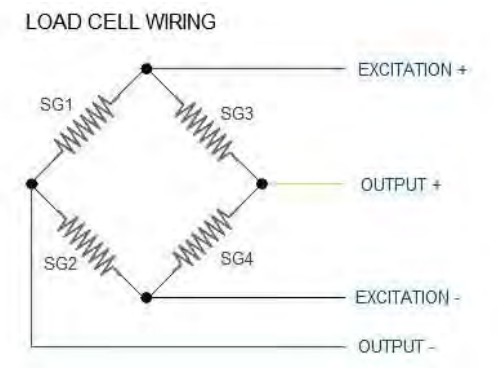
\includegraphics[width=0.35\textwidth]{./gambar/wheatstone_loadcell.png}
        \caption{Wheatstone Bridge Circuit on Load Cell\cite{rahman2018autonomous}.}
        \label{fig:Wheatstone_Bridge}
    \end{figure}
    
    \begin{equation}
      V_{\mathrm{out}} = V_{\mathrm{in}} \cdot \frac{R_2 \cdot R_3 - R_1 \cdot R_4}{(R_1 + R_2) \cdot (R_3 + R_4)}
      \label{eq:Wheatstone_Bridge}
    \end{equation}
    
    \hspace*{1em} Inside the Load Cell Sensor, the system is equipped with a Wheatstone Bridge circuit. The Wheatstone Bridge, as shown in Figure \ref{fig:Wheatstone_Bridge}, is a circuit used to measure resistance changes with high sensitivity \cite{rahman2018autonomous}. To measure the resistance changes, the Wheatstone Bridge equation is used as in Equation \ref{eq:Wheatstone_Bridge}. 

    \item \textit{Real Time Operating System} (RTOS)
    \label{subsec:rtos}

    \hspace*{1em} The Real-Time Operating System (RTOS) is an essential component in modern embedded systems. Its ability to effectively manage concurrent tasks allows the system to process data from various sensors, such as load cells, simultaneously, and control actuators with high precision \cite{sayyad2023real}. RTOS allows the system to perform multiple tasks simultaneously, prioritizing more important tasks \cite{digikey2021task}. This enables the robot to respond quickly to environmental changes, such as maintaining balance, and overall improves the performance and adaptability of robotics using embedded systems.

    \item PID Control System
    \label{subsec:sistemkontrolpid}

    \hspace*{1em} The use of a PID (Proportional-Integral-Derivative) control system is a common method used in servo motor control. This system helps maintain the balance and stability of the robot by correcting movements based on the error values generated from the difference between the actual position and the desired position. PID consists of three main components: proportional control (P), integral control (I), and differential control (D). Each of these components functions to correct errors in different ways.

    \hspace*{1em} The combination of these three components forms an effective PID control in maintaining the balance and stability of the robot. Proper adjustment of the $K_p$, $K_i$, and $K_d$ parameters is crucial to ensure the system performs optimally and responsively.

    \begin{equation}
      \mathrm{Correction} = K_p \cdot \mathrm{error} + K_i \cdot \int_{0}^{t} \mathrm{error} \cdot dt + K_d \cdot \frac{d\mathrm{error}}{dt}
    \end{equation}

    \item Center of Pressure
    \label{subsec:pusattekanan}

    \hspace*{1em} The center of pressure is the point where all forces are concentrated without any torque moment \cite{hawley2016external}. In this center of pressure, several pressures are calculated based on the cross-sectional area to obtain the position of the center of pressure. The Center of Pressure is related to the balance of the robot, especially at the center of gravity \cite{arifin2017implementasi}.

    \begin{equation}
      X_{\mathrm{cop}} = X_0 + \frac{(F2 + F4) \cdot dx}{F1 + F2 + F3 + F4}
      \label{eq:COP_X_1}
    \end{equation}

    \begin{equation}
      Y_{\mathrm{cop}} = Y_0 + \frac{(F1 + F2) \cdot dy}{F1 + F2 + F3 + F4}
      \label{eq:COP_Y_1}
    \end{equation}


    \begin{figure} [h] \centering
      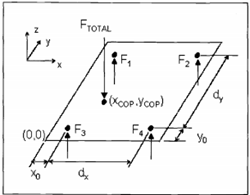
\includegraphics[width=0.3\textwidth]{gambar/Konsep_Letak.png}
      \caption{Concept of Pressure Sensor Placement\cite{resna2005}.}
      \label{fig:Konsep_Letak}
    \end{figure}

    \hspace*{1em} Figure \ref{fig:Konsep_Letak} shows the concept of pressure sensor placement. From this concept, the center of pressure can be calculated using Equations \ref{eq:COP_X_1} and \ref{eq:COP_Y_1}.
\end{enumerate}
